\section{拟解决的科学问题}

立项依据的分析表明，精细排序制度通过评审者的保守偏差与申请者的策略响应形成自我强化的负向循环，而"合格筛选+部分随机"机制可能从规则层面打破这一循环。本项目围绕"规则—心理机制—行为反应"的因果链条，将上述判断分解为以下三个可检验的科学问题。

\noindent\textbf{Q1：评审者行为——排序压力如何塑造评审偏差？机制转换能否缓解？}

在评审噪声不可避免的条件下，精细排序是否会通过放大损失厌恶与认知负荷，诱发更强的保守倾向与对"安全信号"的依赖？若将评审任务从"排序"转为"合格筛选"，这些偏差是否得到缓解？本问题将比较两种规则下的评分分布、对高风险提案的评价差异以及评审一致性，并通过测量认知负荷、损失厌恶与负面信息权重等中介变量，揭示偏差缓解的心理机制。同时，本问题还将考察评审用时、分歧程度、评审理由质量与评分稳定性等效率指标的变化，并识别效率改善的来源——是源于减少了边际比较的认知成本，还是降低了策略性评分的动机。

\noindent\textbf{Q2：申请者行为——机制转换如何改变选题风险与努力配置？}

当资助规则从"排序竞争"转向"合格准入+抽签机会"时，申请者的参照点是否由"击败对手"转向"达到阈值"，其损失厌恶与风险权重是否发生系统性变化？这种心理转变是否会导致更少的包装性投入与更高的探索性选题比例？本问题将比较两种规则下申请者的风险选题比例以及包装性投入与实质性投入的配置变化，并通过测量参照点转移（击败对手vs.达标机会）和风险感知与损失权重变化等机制变量，揭示行为调整的心理基础。

\noindent\textbf{Q3：成果结构——机制转换能否改善资助组合的创新多样性？其最优设计参数的边界条件是什么？}

本问题在Q1和Q2的行为证据基础上，考察资助组合层面的结构性指标（创新多样性、风险型项目占比、总体效率），并进一步识别不同设计参数组合（随机比例、合格阈值、程序透明度与问责机制）对上述指标的影响，确定机制优化的边界条件。

% \section{研究目标}

% 本项目以行为经济学与机制设计理论为基础，通过理论建模与实验检验相结合的主线方法，辅以文献计量、智能体仿真（ABM）和问卷调查，系统回答上述三个科学问题。具体研究目标包括：

% （1）构建整合信号检测、竞赛理论与验证成本理论的统一理论框架，推导排序竞争与合格筛选+抽签两种机制下评审者与申请者的行为均衡，生成可检验预测（P1—P3）。

% （2）通过系列可控实验因果识别机制转换的行为效应：实验室实验在激励兼容的抽象环境中检验核心预测；田野实验（或准自然实验）在真实资助情境中验证生态效度。

% （3）通过辅助方法为主线研究提供支撑：文献计量提供模型参数校准与国际证据基线；ABM仿真探索设计参数的长期动态效应；问卷调查建立科研人员风险偏好与参照点的基线特征。

% （4）识别部分随机机制实现"效率—创新—程序正当性"兼容的边界条件与最优设计参数，为科研资助改革提供可操作的证据基础。

\section{研究方法}

本项目以理论建模与实验检验为主线方法，辅以文献计量、基于主体的仿真（Agent-Based Modeling,以下简称ABM仿真）和问卷调查三种支撑方法，系统回答上述三个科学问题。理论建模用于刻画关键机制并形成可检验预测；实验模块在控制环境下识别因果机制，并在真实情境中检验外部效度。文献计量为关键参数提供经验校准与情境参照，问卷调查提供偏好与异质性基线设定。实验效应量用于校准ABM仿真的行为规则，ABM仿真的长期预测与参数空间探索反向为实验与田野环节提供参数选取与机制设计依据，从而形成可迭代的证据闭环。研究方法总体框架如图1所示。

\begin{figure}[h!]
	\centering %图片居中
	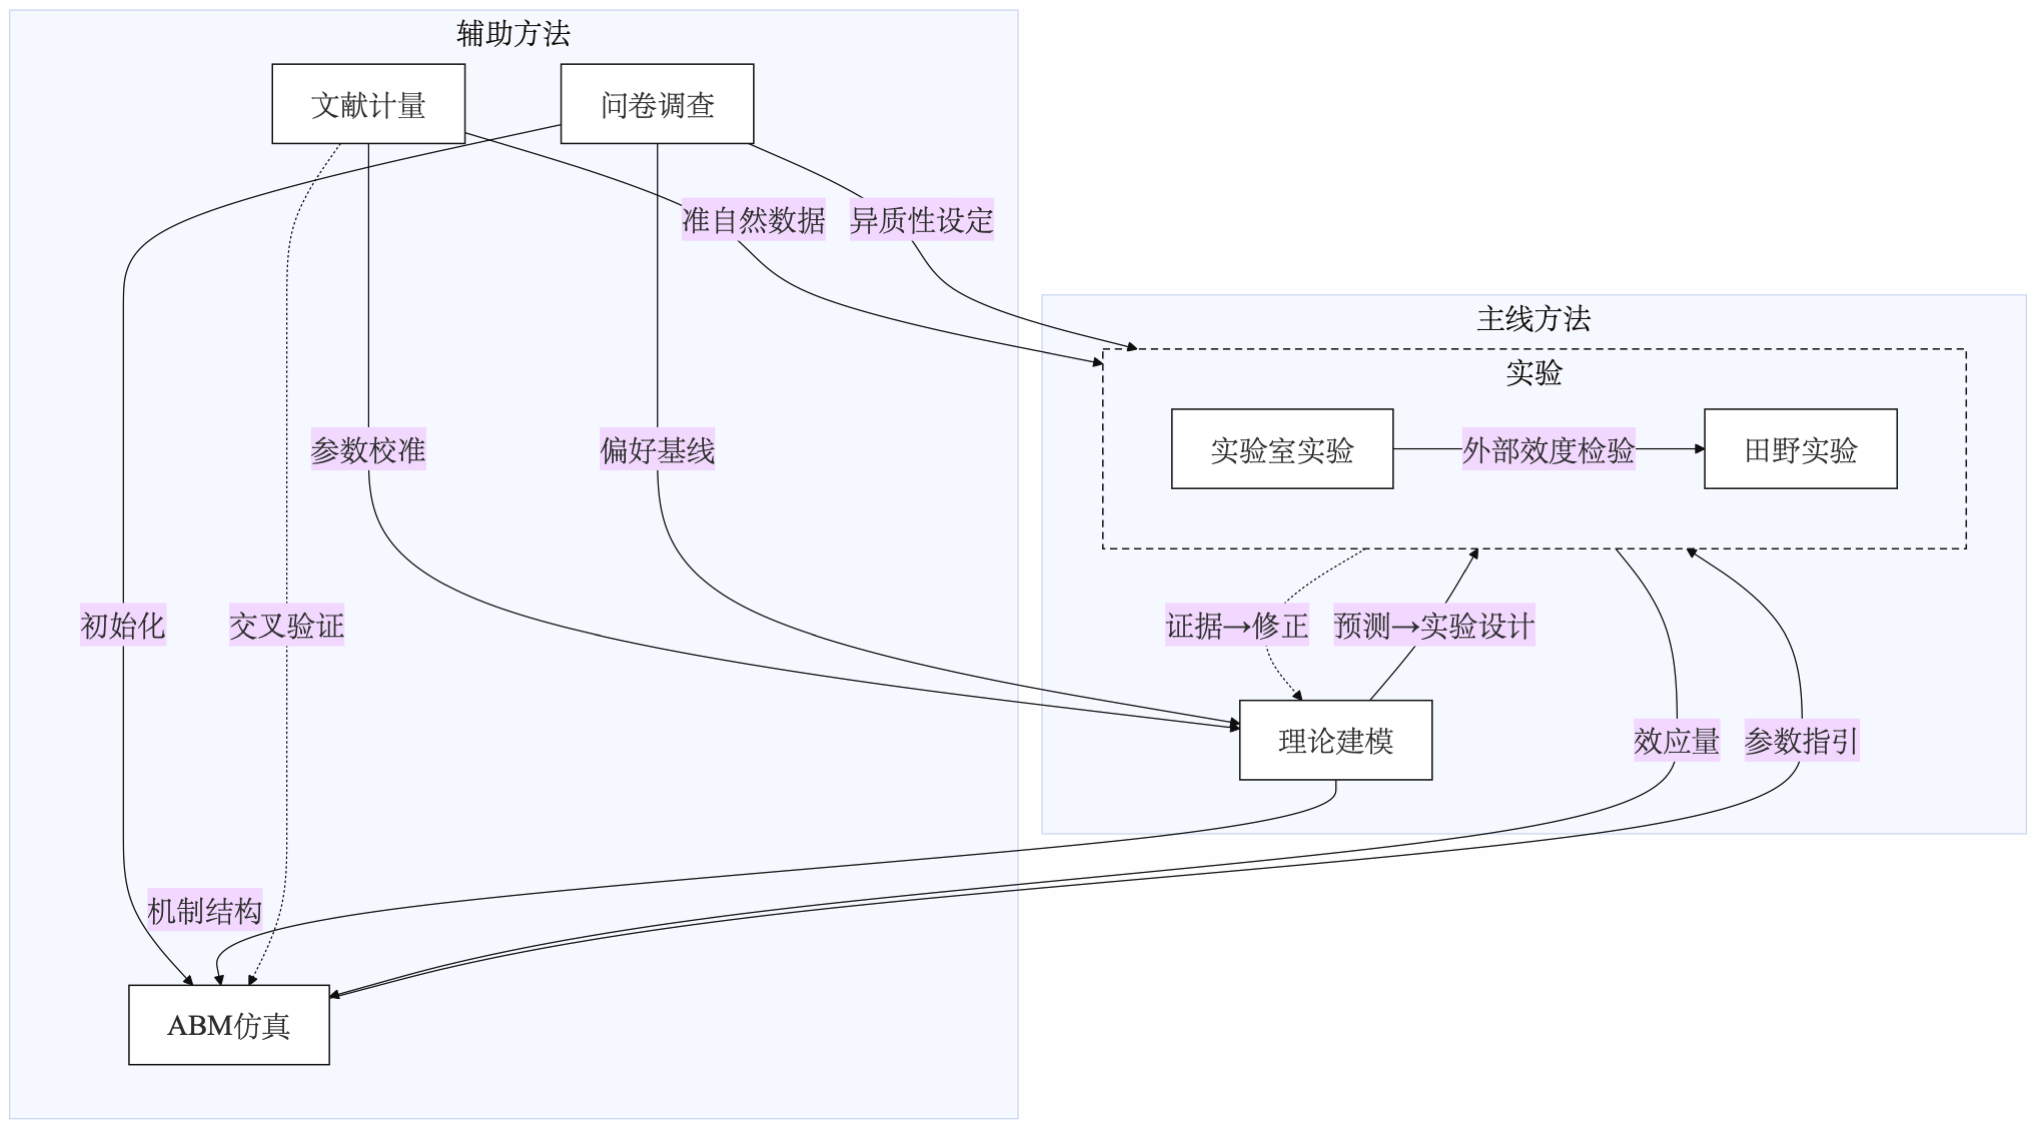
\includegraphics[width=\textwidth]{figures/methods.png}
	\captionsetup{justification=centering} %图题居中
	\caption{多方法融合的研究设计框架}
\end{figure}

\subsection{理论建模：评审者与申请者的行为博弈模型}

本项目拟构建一个双边博弈模型，用以刻画科研资助过程中“文书打磨—评审决策—项目选择”三者之间的相互作用。本节提出“基础模型”，旨在在一组自然且可解释的充分条件下，提出一组直观、可检验的比较静态结论。为兼顾申请书篇幅与可读性，本节仅报告直觉化的解释。后续正式研究将在此基础上扩展模型结构，并给出严格的数学证明与数值验证。


% \textbf{基本模型设定} \quad 考虑一个科研资助机构、$N$ 个潜在项目申请人以及 $M$ 名评审专家。每位申请人 $i$ 拥有一个研究项目，其内在科研质量记为 $\theta_i$，反映项目的真实科研潜力。$\theta_i$ 服从已知分布 $F(\theta)$，密度为 $f(\theta)$，支撑在 $[\underline{\theta}, \bar{\theta}]$ 上，并在申请阶段被视为外生给定。

% 申请人在提交申请时，可在研究计划书的撰写与打磨上投入努力 $e_i \ge 0$（表述优化、结构组织、可行性呈现等）。文书投入不改变项目真实科研质量 $\theta_i$，而仅影响评审专家观察到的项目信号。文书投入成本为 $\psi(e_i)=\frac{\gamma}{2}e_i^2$，$\gamma>0$。

% 为刻画项目类型选择，引入Manso（2011）关于探索与利用权衡的思想。申请人可选择安全型项目（$\kappa_i=S$）或风险型项目（$\kappa_i=R$）。风险型项目在评审中面临系统性不利——其研究路径的不确定性更难被文书充分呈现、更易被评审认为可行性不足（Boudreau等, 2016; Lane等, 2022），令评审观察到的有效信号为

% \begin{equation}
%     \tilde{s}_i=\theta_i+e_i-\delta\cdot\mathbf{1}\{\kappa_i=R\}+\varepsilon_i,\quad \delta>0,
% \end{equation}

% 其中 $\varepsilon_i\sim\mathcal{N}(0,\sigma^2)$ 表示评审噪声（主观判断、时间约束、匹配度等因素导致）。若项目获得资助，其资助后的期望科学价值为 $V_S=p_sR_s$（安全型）与 $V_R=p_rR_r$（风险型）。


% \textbf{资助机制} \quad 本文比较两种资助机制 $m\in\{T,L\}$，均基于有效信号 $\tilde{s}_i$ 作出决策。

% 传统排序机制（T）。 评审专家基于 $\tilde{s}_i$ 对所有申请项目进行排序，资助得分最高的 $K$ 个项目。大样本下等价于存在一个隐含截止分数 $s_T^*$，使得

% $$\Pr(\tilde{s}_i\ge s_T^*)=\frac{K}{N}. $$

% 部分随机资助机制（L）。 评审专家设定阈值 $\tau$，仅判断项目是否达到基本科研标准。所有满足 $\tilde{s}_i\ge \tau$ 的项目进入"合格池"，最终在合格池内随机抽签确定 $K$ 个资助对象。该机制将评审任务从Ben-Porath等（2014）意义上的"完全排序+逐一验证"简化为"阈值筛选+随机分配"，从而降低了验证成本。令项目进入合格池的概率为

% $$q(\theta,e,\kappa;\tau)=1-\Phi\!\left(\frac{\tau-\theta-e+\delta\mathbf{1}\{\kappa=R\}}{\sigma}\right). $$

% 在对称均衡下，记平均过线概率为 $\bar{q}(\tau)$。当合格池期望规模 $N\bar{q}(\tau)\ge K$ 时，条件于过线的中签概率近似为

% $$\pi(\tau)=\frac{K}{N\bar{q}(\tau)}\in(0,1]. $$

% A1（大样本价格接受）：$N$ 较大，单个申请人的 $e_i$ 对 $\bar{q}(\tau)$ 的影响可忽略。因此对单个申请人而言，$\pi(\tau)$ 可视为常数，且不随其 $e_i$ 改变。

% （3）申请人的决策问题（条件于参与申请）。 在给定资助机制 $m\in\{T,L\}$ 下，申请人 $i$ 选择项目类型 $\kappa_i\in\{S,R\}$ 与文书投入 $e_i\ge 0$，其期望效用为

% $$U_m(\theta_i,e_i;\kappa_i)=P_m(\theta_i,e_i;\kappa_i)\cdot V_{\kappa_i}-\frac{\gamma}{2}e_i^2-c, $$

% 其中 $P_m(\cdot)$ 表示在机制 $m$ 下获得资助的概率。

% （4）排序机制下的最优文书投入。 排序机制下获得资助当且仅当 $\tilde{s}\ge s_T^*$，因此

% $$P_T(\theta,e;\kappa)=1-\Phi\!\left(\frac{s_T^*-\theta-e+\delta\mathbf{1}\{\kappa=R\}}{\sigma}\right). $$

% 对 $e$ 求一阶条件（FOC）得到最优文书投入 $e_T^*(\theta,\kappa)$ 满足：

% $$\gamma e_T^*(\theta,\kappa)=\frac{V_\kappa}{\sigma}\phi\!\left(\frac{s_T^*-\theta-e_T^*(\theta,\kappa)+\delta\mathbf{1}\{\kappa=R\}}{\sigma}\right). $$

% 其中 $\Phi(\cdot)$ 与 $\phi(\cdot)$ 分别表示标准正态分布函数与密度函数。为确保 $e_T^*$ 的唯一性，可施加温和的充分条件（如 $\gamma$ 足够大），使一阶条件的零点唯一。正式研究中将给出严格的充分条件与证明。

% （5）部分随机机制下的最优文书投入。 在部分随机机制下，资助概率为 $P_L(\theta,e;\kappa;\tau)=q(\theta,e,\kappa;\tau)\cdot\pi(\tau)$。由一阶条件得到 $e_L^*(\theta,\kappa;\tau)$ 满足：

% $$\gamma e_L^*(\theta,\kappa;\tau)=\pi(\tau)\frac{V_\kappa}{\sigma}\phi\!\left(\frac{\tau-\theta-e_L^*(\theta,\kappa;\tau)+\delta\mathbf{1}\{\kappa=R\}}{\sigma}\right). $$

% （6）核心命题（直觉证明要点）。 基于上述模型分析，推导以下核心命题：

% \begin{proposition}
%     （部分随机机制弱化文书军备竞赛）。 在可比筛选强度下（例如令 $\tau=s_T^*$ 使两机制边际标准一致），且合格池使 $\pi(\tau)\in(0,1)$，对任意给定 $(\theta,\kappa)$，
%  $$e_L^*(\theta,\kappa;\tau) < e_T^*(\theta,\kappa).$$
% \end{proposition}

% 证明要点。 在 $\tau=s_T^*$ 下，两机制的"过线概率"对 $e$ 的边际响应相同，而部分随机机制的资助概率为 $P_L=\pi(\tau)\,q(\cdot)$，其中 $\pi(\tau)\in(0,1)$ 且对单个申请人而言不随其 $e$ 变化（A1）。因此对任意 $e$，$\frac{\partial P_L}{\partial e}=\pi(\tau)\frac{\partial P_T}{\partial e}$，即部分随机机制的边际收益在所有 $e$ 上都被严格缩放为排序机制的 $\pi(\tau)$ 倍。由于两机制的边际成本均为 $\gamma e$ 且严格递增，满足一阶条件"边际收益=边际成本"的最优 $e$ 在部分随机机制下必然严格更小，从而得到 (9)。$\blacksquare$

% 该命题揭示了部分随机机制弱化文书军备竞赛的核心机制：排序制下文书投入的边际回报取决于相对排名的微小优势，竞争激烈时边际回报可观，诱导过度投入；而部分随机机制中，一旦信号超过阈值 $\tau$，额外文书投入仅提高过线概率但不影响中签概率 $\pi(\tau)$，边际回报被打折因子 $\pi(\tau) < 1$ 系统性削弱，从而抑制了"包装竞赛"。

% \begin{proposition}
%     （部分随机机制更有利于风险型项目的选择）。 在给定 $(\theta,\kappa)$ 的最优文书投入由(7)—(8)确定的基础上，申请人进一步比较两类型在机制 $m$ 下的最大化后效用 $W_m(\theta,\kappa)\equiv \max_{e\ge 0}U_m(\theta,e;\kappa)$。在下列充分条件下——(i)先选题后投入；(ii)高回报优势 $V_R-V_S$ 足够大；(iii)呈现折扣 $\delta$ 中等（不过大亦不可忽略）；(iv)可比筛选强度与合格池抽签公平——存在一段内在质量区间 $\Theta\subset[\underline{\theta},\bar{\theta}]$，使得

%  $$\kappa_T^*(\theta)=S,\quad \kappa_L^*(\theta)=R,\quad \forall\theta\in\Theta, $$
%   从而总体上风险型选择比例在部分随机机制下更高：$\Pr(\kappa=R\mid L)>\Pr(\kappa=R\mid T)$。
% \end{proposition}

% 证明要点。 排序机制中，风险折扣 $\delta$ 会持续作用于"边际排序竞争"，显著压低风险型项目的最优资助概率与最大化后效用 $W_T(\theta,R)$；而部分随机机制中，一旦达标进入合格池，中签概率与信号高低无关，使风险折扣不再在达标后的"二次排序阶段"被放大。故相对排序机制，部分随机机制提高了风险型项目的相对回报 $W_L(\theta,R)-W_L(\theta,S)$。当 $V_R-V_S$ 足够大且 $\delta$ 处于中等水平时，存在一段边际质量区间 $\Theta$ 使最优类型由安全型转为风险型，从而推出 (10)。$\blacksquare$

% \begin{proposition}
%     （高噪声下部分随机机制的效率优势）。 定义两机制的社会福利：

%  $$SW_T = K\cdot\mathbb{E}[V_\kappa\mid \tilde{s}\ge s_T^*] - Mc_{\text{review}} - \eta g(s_T^*) - \mathbb{E}\!\left[\frac{\gamma}{2}(e_T^*)^2+c\right], $$

%  $$SW_L(\tau) = K\cdot\mathbb{E}[V_\kappa\mid \tilde{s}\ge \tau] - Mc_{\text{review}} - \mathbb{E}\!\left[\frac{\gamma}{2}(e_L^*)^2+c\right], $$

%  其中 $\eta g(s_T^*)$ 表示排序制下精细排序的额外认知成本（与截止点附近的拥挤度/不可区分性单调相关；噪声越高、边际越拥挤，精细排序成本越大）。在下列充分条件下——(i)高噪声降低排序信息含量：$\sigma^2$ 上升使条件期望优势递减；(ii)精细排序成本随不可区分性上升；(iii)命题1保证 $e_T^*>e_L^*$，排序制引致更高的努力浪费——存在阈值 $\bar{\sigma}^2$，使得当 $\sigma^2\ge\bar{\sigma}^2$ 时，

%  $$\max_\tau SW_L(\tau) > SW_T. $$
% \end{proposition}

% 证明要点。 随着 $\sigma^2$ 增大，排序机制在边际区间的精细比较越来越由噪声驱动，排序的"信息增益"递减；同时截止附近不可区分性增强使额外认知成本 $\eta g(s_T^*)$ 上升，并且排序机制诱导更强的文书军备竞赛（命题1）带来更高的努力浪费。部分随机机制以"达标筛选"为主，避免在高噪声区间进行低信息含量的精细排序，并通过降低文书投入减少无效成本。因此在 $\sigma^2$ 足够大时，存在最优阈值 $\tau$ 使得节约的排序认知成本与努力浪费超过潜在的选择精度损失，从而总体福利严格更高，得到 (13)。$\blacksquare$

% （7）可检验预测（对应实验设计）。 上述命题直接生成以下可检验预测：P1（文书投入）——在可比筛选强度下，部分随机机制显著降低文书投入 $e$（命题1）；P2（风险选择）——在 $V_R-V_S$ 较大且 $\delta$ 中等时，部分随机机制提高风险型项目选择比例（命题2）；P3（噪声异质性）——当评审噪声更高（时间压力/信息更少/匹配度更差），部分随机机制的相对福利优势更显著（命题3）。这三条预测将直接映射为实验室实验（2.2.1节）中的处理效应假说，均衡效应量预测将为检验力分析提供依据。ABM仿真（2.4节）也将以本模型的均衡策略与行为规则为基础构建智能体决策函数。
\subsubsection{模型的基本设定}
考虑一个科研资助机构与 $N$ 个潜在申请人。每位申请人 $i$ 拥有一个研究项目，其\emph{内在科研质量}为 $\theta_i\in[\underline{\theta},\bar{\theta}]$，在申请阶段视为外生给定，服从已知分布 $F(\theta)$。

申请人可在申请书撰写与打磨上投入努力 $e_i\ge 0$（如表述优化、结构组织、可行性呈现等）。该投入\emph{不改变}项目真实科研质量 $\theta_i$，仅影响评审可观察到的项目信号；投入成本为
\begin{equation}
    \psi(e_i)=\frac{\gamma}{2}e_i^2,\quad \gamma>0 .
\end{equation}

申请人可选择项目类型 $\kappa_i\in\{S,R\}$（安全型/风险型）。风险型项目在评审中面临系统性不利（如更难呈现路径确定性、更易被认为可行性不足），用“呈现折扣” $\delta>0$ 表示。评审对项目形成的\emph{有效信号}定义为
\begin{equation}
    s_i=\theta_i+e_i-\delta\cdot\mathbf{1}\{\kappa_i=R\}+\varepsilon_i,\quad 
    \varepsilon_i\sim\mathcal{N}(0,\sigma^2),\ \delta>0 .
    \label{eq:signal}
\end{equation}
其中 $\varepsilon_i$ 表示评审噪声（主观判断、时间约束、匹配度等导致）。 评审最终用于决策的评分可以表示为某个函数 $G(s)$，且满足单调性：若 $s_i>s_j$ 则 $G(s_i)>G(s_j)$。
因此在不损失一般性的前提下，可直接以 $s$ 表示评审用于排序/过线判断的有效评分信号。

若项目获得资助，其对申请人的期望价值记为 $V_\kappa$，并允许 $V_R>V_S$ 以反映“高风险高收益”的科研产出结构。

\subsubsection{两种资助机制}
比较两种机制 $m\in\{T,L\}$，均基于有效信号 $s_i$ 作出资助决策，资助名额为 $K$。

\textbf{机制 $T$：传统精细排序（Top-$K$）}\quad
评审按 $s$ 对申请排序，资助得分最高的 $K$ 个项目。大样本下等价于存在隐含截止分数 $s_T^*$，使得
\begin{equation}
    \Pr(s_i\ge s_T^*)=\frac{K}{N}.
    \label{eq:cutoff}
\end{equation}
在本基础模型中，将 $s_T^*$ 视为由资助强度/预算与总体竞争环境决定的外生政策参数。

\textbf{机制 $L$：阈值准入 + 合格池抽签（部分随机）}\quad
评审设定阈值 $\tau$，仅判断项目是否达标。所有满足 $s_i\ge\tau$ 的项目进入“合格池”，最终在合格池内随机抽签确定 $K$ 个资助对象。给定 $(\theta,e,\kappa)$ 的过线概率为
\begin{equation}
    q(\theta,e,\kappa;\tau)=\Pr(s\ge\tau)
    =1-\Phi\!\left(\frac{\tau-\theta-e+\delta\mathbf{1}\{\kappa=R\}}{\sigma}\right),
    \label{eq:q}
\end{equation}
其中 $\Phi(\cdot)$ 为标准正态分布函数。记对称情形下总体平均过线概率为 $\bar q(\tau)$。当合格池期望规模 $N\bar q(\tau)\ge K$ 时，条件于过线的中签概率为
\begin{equation}
    \pi(\tau)=\frac{K}{N\bar q(\tau)}\in(0,1].
    \label{eq:pi}
\end{equation}
当 $N$ 足够大时，单个申请人的 $e_i$ 对 $\bar q(\tau)$ 的影响可忽略，因此对个体而言 $\pi(\tau)$ 可视为常数，且不随其 $e_i$ 改变。

\subsubsection{申请人的决策问题}

给定机制 $m\in\{T,L\}$，申请人选择项目类型 $\kappa\in\{S,R\}$ 与文书投入 $e\ge 0$，其期望效用为
\begin{equation}
    U_m(\theta,e;\kappa)=P_m(\theta,e;\kappa)\cdot V_\kappa-\frac{\gamma}{2}e^2-c,
    \label{eq:utility}
\end{equation}
其中 $P_m(\cdot)$ 为机制 $m$ 下获得资助的概率，$c$ 为固定申请成本。

\textbf{机制 $T$ 下的资助概率与最优投入}\quad
在机制 $T$ 下，获得资助当且仅当 $s\ge s_T^*$，因此
\begin{equation}
    P_T(\theta,e;\kappa)=1-\Phi\!\left(\frac{s_T^*-\theta-e+\delta\mathbf{1}\{\kappa=R\}}{\sigma}\right).
    \label{eq:PT}
\end{equation}
若最优解为内点 $e_T^*(\theta,\kappa)>0$，则一阶条件为
\begin{equation}
    \gamma e_T^*(\theta,\kappa)=\frac{V_\kappa}{\sigma}\,
    \phi\!\left(\frac{s_T^*-\theta-e_T^*(\theta,\kappa)+\delta\mathbf{1}\{\kappa=R\}}{\sigma}\right),
    \label{eq:FOC_T}
\end{equation}
其中 $\phi(\cdot)$ 为标准正态密度函数。

\textbf{机制 $L$ 下的资助概率与最优投入}\quad
在机制 $L$ 下，资助概率为“过线 $\times$ 中签”
\begin{equation}
    P_L(\theta,e;\kappa;\tau)=q(\theta,e,\kappa;\tau)\cdot \pi(\tau).
    \label{eq:PL}
\end{equation}
若最优解为内点 $e_L^*(\theta,\kappa;\tau)>0$，则一阶条件为
\begin{equation}
    \gamma e_L^*(\theta,\kappa;\tau)=\pi(\tau)\frac{V_\kappa}{\sigma}\,
    \phi\!\left(\frac{\tau-\theta-e_L^*(\theta,\kappa;\tau)+\delta\mathbf{1}\{\kappa=R\}}{\sigma}\right).
    \label{eq:FOC_L}
\end{equation}
为使最优文书投入具有良好比较静态（并避免多重内点），假设对任意给定 $(\theta,\kappa)$，
机制 $m\in\{T,L\}$ 下的最优文书投入 $e_m^*(\theta,\kappa)$ 唯一（例如可由“$\gamma$ 足够大”保证；正式研究中将给出严格充分条件与证明）。


\subsubsection{核心命题}

\begin{proposition}
（部分随机机制弱化文书军备竞赛）
在可比筛选强度下（例如令阈值 $\tau$ 使合格池期望规模为 $\lambda K$，其中 $\lambda>1$，
即 $N\bar q(\tau)=\lambda K$，从而 $\pi(\tau)=1/\lambda\in(0,1)$；并将排序制的 Top-$K$ 截止点 $s_T^*$ 由
$\Pr(s\ge s_T^*)=K/N$ 确定），对任意给定 $(\theta,\kappa)$，有
\begin{equation}
    e_L^*(\theta,\kappa;\tau) < e_T^*(\theta,\kappa).
    \label{eq:prop1}
\end{equation}
\end{proposition}
\noindent\textbf{直觉解释} \quad 
部分随机机制把“获资助”的边际回报整体乘上折扣因子 $\pi(\tau)\in(0,1)$：超过阈值后，额外文书投入只提高过线概率而不改变中签概率，因此文书投入的边际收益被系统性削弱。
在边际成本 $\gamma e$ 不变且递增的情况下，最优投入点必然左移，从而 $e_L^*<e_T^*$。$\blacksquare$

% \noindent\textbf{证明要点} \quad
% 固定 $(\theta,\kappa)$。在机制 $T$ 下，资助概率为 $P_T(\theta,e;\kappa)$；在机制 $L$ 下，$P_L(\theta,e;\kappa;\tau)=\pi(\tau)\,q(\theta,e,\kappa;\tau),$
% 其中 $\pi(\tau)\in(0,1)$ 且由 A1 对单个申请人而言不随其 $e$ 变化。
% 在“可比筛选强度”设定下，阈值筛选的边际标准与排序制的边际标准对齐（可理解为将 $\tau$ 选取在 $s_T^*$ 附近，
% 使得在相关边际区间内 $q(\theta,e,\kappa;\tau)$ 与 $P_T(\theta,e;\kappa)$ 对 $e$ 的边际响应一致）。
% 因此对任意 $e$，$\frac{\partial P_L}{\partial e}=\pi(\tau)\frac{\partial P_T}{\partial e},$即部分随机机制下的边际收益在所有 $e$ 上都被严格缩放为排序机制的 $\pi(\tau)$ 倍。
% 两机制的边际成本同为 $\gamma e$ 且严格递增；在 A2（最优解唯一）下，
% “边际收益=边际成本”的唯一交点在边际收益整体下移时必然严格左移，
% 从而最优文书投入满足 $e_L^*(\theta,\kappa;\tau)<e_T^*(\theta,\kappa)$，得到 \eqref{eq:prop1}。\ $\blacksquare$

\begin{proposition}
（部分随机机制更有利于风险型项目的选择）
令最大化后效用为
\[
W_m(\theta,\kappa)\equiv \max_{e\ge 0}U_m(\theta,e;\kappa),\qquad 
\Delta W_m(\theta)\equiv W_m(\theta,R)-W_m(\theta,S).
\]
在如下条件下： (i) 先选题后投入；(ii) $\Delta W_m(\theta)$ 关于 $\theta$ 满足单交叉（随 $\theta$ 严格递增）；
(iii) 选择 $\tau$ 使合格池规模为 $\lambda K$（$\lambda>1$），从而 $\pi(\tau)=1/\lambda\in(0,1)$ 且 $\tau<s_T^*$；
(iv) $V_R>V_S$ 且 $\delta>0$（风险型存在呈现折扣），
则存在一段非空区间 $\Theta\subset[\underline{\theta},\bar{\theta}]$ 使得
\[
\kappa_T^*(\theta)=S,\quad \kappa_L^*(\theta)=R,\quad \forall\theta\in\Theta,
\]
从而总体上风险型选择比例在部分随机机制下更高：$\Pr(\kappa=R\mid L)>\Pr(\kappa=R\mid T)$。
\end{proposition}

% \noindent\textbf{证明要点。}\ 
% 比较两机制下风险折扣 $\delta$ 对“达标概率”的影响。对任意给定 $(\theta,e)$，
% 机制 $T$ 的达标阈值为 $s_T^*$，机制 $L$ 的达标阈值为 $\tau<s_T^*$。
% 由于风险型信号相对安全型左移 $\delta$，其达标概率损失为
% \[
% \Delta(t)\equiv \Pr(s\ge t\mid S)-\Pr(s\ge t\mid R)
% =\Phi\!\left(\frac{t-(\theta+e)+\delta}{\sigma}\right)-\Phi\!\left(\frac{t-(\theta+e)}{\sigma}\right),
% \]
% 且该损失随阈值 $t$ 上升而加大（阈值越高，尾部切割越“尖”，同样的平移 $\delta$ 造成的过线概率损失越大）。
% 因此在相同 $(\theta,e)$ 下，风险型在机制 $T$ 面临的相对概率劣势强于机制 $L$（因为 $s_T^*>\tau$）。
% 再结合命题1给出的 $e_L^*<e_T^*$（部分随机机制降低文书投入与努力浪费），可得风险型相对安全型的最大化后效用差
% $\Delta W_L(\theta)$ 相对 $\Delta W_T(\theta)$ 向上移动。
% 在单交叉条件下，存在一段边际质量区间 $\Theta$ 使得机制 $T$ 下仍选安全型而机制 $L$ 下转而选择风险型，从而风险型占比在 $L$ 下更高。\ $\blacksquare$


\noindent\textbf{直觉解释} \quad 
风险型项目的劣势来自“呈现折扣” $\delta$ 导致信号左移；排序制的 Top-$K$ 截止点更高，尾部筛选会放大这一下移带来的过线概率损失，而部分随机机制采用更低的达标阈值 $\tau<s_T^*$，从而减轻风险折扣的惩罚。再叠加命题1所示文书军备竞赛被抑制（努力浪费更少），风险型在一段边际质量区间内更可能成为最优选择。$\blacksquare$

\begin{proposition}
（高噪声下部分随机机制的效率优势）
将两种机制下的社会福利定义为“科学产出收益”减去“评审成本”与“申请成本”：
\begin{align}
SW_T
&=
K\cdot\mathbb{E}\!\left[V_\kappa \mid s\ge s_T^*\right]
-\underbrace{C_T(\sigma,s_T^*)}_{\text{精细排序的认知/时间成本}}
-\mathbb{E}\!\left[\frac{\gamma}{2}\big(e_T^*(\theta,\kappa)\big)^2+c\right],
\label{eq:SWT_new}
\\
SW_L(\tau)
&=
K\cdot\mathbb{E}\!\left[V_\kappa \mid s\ge \tau\right]
-\underbrace{C_L(\sigma,\tau)}_{\text{阈值筛选成本}}
-\mathbb{E}\!\left[\frac{\gamma}{2}\big(e_L^*(\theta,\kappa;\tau)\big)^2+c\right],
\label{eq:SWL_new}
\end{align}
其中 $s_T^*$ 为 Top-$K$ 截止点（$\Pr(s\ge s_T^*)=K/N$），$\tau$ 为准入阈值；
且 $C_T(\sigma,s_T^*)-C_L(\sigma,\tau)$ 随评审噪声 $\sigma$ 上升而（弱）增大，反映高噪声下精细区分更困难、更耗时。

若满足以下条件：（i）噪声上升降低精细排序的信息增益（$\sigma^2$ 上升使
$\mathbb{E}[V_\kappa\mid s\ge s_T^*]-\mathbb{E}[V_\kappa\mid s\ge \tau]$ 递减）；
（ii）精细排序成本对噪声更敏感（$C_T-C_L$ 随 $\sigma$ 上升而增大）；
（iii）命题1成立从而 $\mathbb{E}[(e_T^*)^2]>\mathbb{E}[(e_L^*)^2]$（排序制诱导更高努力浪费），
则存在阈值 $\bar\sigma^2$，使得当 $\sigma^2\ge \bar\sigma^2$ 时，
\begin{equation}
\max_{\tau} SW_L(\tau) \;>\; SW_T .
\label{eq:prop3_new}
\end{equation}
\end{proposition}

% \noindent\textbf{证明要点。}\ 
% 随着 $\sigma^2$ 增大，排序机制在边际区间的精细比较越来越由噪声驱动，排序带来的“信息增益”递减；
% 同时截止附近不可区分性增强使额外认知成本 $\eta g(s_T^*,\sigma)$ 上升，
% 并且排序机制诱导更强的文书军备竞赛（命题1）带来更高的努力浪费。
% 部分随机机制以“达标筛选”为主，避免在高噪声区间进行低信息含量的精细排序，并通过降低文书投入减少无效成本。
% 因此当 $\sigma^2$ 足够大时，存在最优阈值 $\tau$ 使得节约的排序认知成本与努力浪费超过潜在的选择精度损失，
% 从而总体福利严格更高，得到 \eqref{eq:prop3}。\ $\blacksquare$

\noindent\textbf{直觉解释} \quad 
当评审噪声较高时，精细排序在边际区间的选优信息含量下降，但认知/时间成本上升且诱发更强的文书军备竞赛；阈值准入+抽签避免在“几乎不可区分”的边际区间做低信息含量排序，并降低无效努力浪费，因此噪声足够大时其福利优势更明显。$\blacksquare$



% \subsubsection{可检验预测}
% P1：在可比筛选强度下，机制 $L$ 显著降低文书投入 $e$（命题1）；

% P2：在 $V_R-V_S$ 较大且 $\delta$ 中等时，机制 $L$ 提高风险型项目选择比例（命题2）；

% P3：当评审噪声更高（如信息更少/时间压力更大），机制 $L$ 的相对福利优势更显著（命题3）。

\subsubsection{后续扩展方向}
在正式研究中，我们将在基础模型之上进一步引入：（a）评审者行为参数——损失厌恶、参考点依赖（前景理论）、负面信息偏差（negativity bias）、锚定与社会信息效应，参考Lane等（2022）关于负面信息对评审保守性影响的实验发现；（b）申请者行为参数——概率加权（对抽签中奖概率的非线性感知）、后悔预期、社会比较偏好；（c）机制内生化——阈值 $\tau$ 的最优化与评审资源约束、不同学科/评审匹配度导致的 $\sigma$ 异质性，参考Adda和Ottaviani（2024）关于评审噪声内生化与Boudreau等（2016）关于智识距离（intellectual distance）影响评审行为的分析框架；（d）时间维度——引入Manso（2011）的多臂老虎机框架，分析部分随机机制对"容忍早期失败"激励的影响。同时，正式研究将对最优解的唯一性给出可检验的充分条件，并在附录中提供命题1—3的严格证明及稳健性分析。

\subsection{实验检验：机制转换的因果识别与效度验证}

通过实验室实验在抽象、可控的激励兼容环境中因果识别配置机制转换对评估者与申请者行为的影响，检验理论模型的核心预测；进而通过田野实验在真实资助情境中验证实验室发现的生态效度（ecological validity），实现从内部效度到外部效度的递进。

\subsubsection{实验室实验：微观机制的因果识别}

本实验采用中性化的抽象框架，不使用“科研资助”“评审”“基金”等情境标签，以避免被试预设的社会偏好或规范效应干扰因果推断。实验仅需满足激励兼容（incentive-compatible）条件：被试的决策与收益直接挂钩，决策环境在结构上与理论模型同构。

采用 2（配置机制：排序竞争 vs. 合格筛选+抽签）× 2（信号噪声：低 vs. 高）的组间设计。每组包含5名"申请者"和1名"评估者"，构成一个完整的配置决策单元。实验包含多轮重复博弈（tentatively 10—15轮），以捕捉学习效应与策略调整。

第一阶段：申请者决策。 每轮开始时，每位申请者面临两个关键决策：

（a）项目类型选择。 申请者在安全型项目（$\kappa=S$）与风险型项目（$\kappa=R$）之间选择。安全型对应收益方差较小、期望值中等的分布；风险型对应收益方差较大、期望值较高但在评估中面临折扣 $\delta$ 的分布。该选择对应模型中的类型选择决策。

（b）时间分配。 申请者在固定总时间内，自主分配时间于两项任务：一项认知任务（如数学推理、模式识别题，模拟实质性研究投入，决定项目真实质量 $\theta_i$）和一项effort task（如限时打字任务，模拟文书打磨投入 $e_i$）。认知任务得分越高，项目真实质量越高；effort task得分越高，文书打磨信号越强。被试须在"提升项目真实质量"与"优化信号呈现"之间进行权衡——这直接对应模型中 $\theta_i$ 与 $e_i$ 的关系。

申请者最终获得一个总分（即评估者观察到的信号 $\tilde{s}_i$），其构成为：安全型总分 $= $ 认知任务得分 $+$ 文书打磨得分 $+$ 随机成分 $\varepsilon_i$；风险型总分 $= $ 认知任务得分 $+$ 文书打磨得分 $- \delta +$ 随机成分 $\varepsilon_i$。随机成分 $\varepsilon_i$ 由计算机抽取，标准差在低噪声与高噪声条件下分别设定。

第二阶段：评估者决策。 评估者观察本组5名申请者的总分（但不知道各成分的具体构成），在不同机制条件下执行不同任务：排序竞争条件下，评估者对5人进行完整排序，排名前 $K$ 位获得"资助"；合格筛选+抽签条件下，评估者仅判断每人是否"达标"（合格/不合格），合格者进入抽签池，由计算机随机确定 $K$ 名"资助"对象。

第三阶段：结果反馈与事后测量。 系统根据机制规则生成结果并反馈各方收益。获得"资助"的申请者，其认知任务得分（代表项目真实质量）按比例兑换为现金奖励；评估者的报酬与其所选对象的认知任务得分挂钩，确保评估者有动机选出真实质量最高的申请者。每轮结束后收集事后测量：公平感知、归因模式、继续参与意愿。

关键测量变量。

- 申请者侧（主要变量）： 安全型 vs. 风险型选择比例（对应预测P2）、认知任务与effort task的时间分配比例（对应预测P1）、认知任务实际得分（实质质量）；
- 评估者侧： 评估用时（对应认知负荷）、风险型项目的排名/通过率（对应预测P2）；
- 系统层面： 获"资助"项目的平均认知任务得分、风险型项目占比、总体效率（对应预测P3）。

激励机制。仅获得"资助"的申请者，其认知任务得分兑换为现金奖励（确保申请者有动机在实质质量与信号包装之间做出真实权衡）。评估者的报酬与被资助者的认知任务得分正相关（确保评估者有动机进行认真评估）。所有被试额外获得固定出场费。

样本量初步估算与检验力分析安排。 根据2×2组间设计，初步计划每个处理单元（cell）包含约15—20个独立session（每session 6人），总样本量约360—480人。由于目前尚未进行正式的检验力分析（power analysis），上述估算基于同类实验经济学研究（如Ederer和Manso, 2013; Charness和Grieco, 2019）的样本量参照。正式的检验力分析将在预实验（pilot）完成后，基于pilot数据的效应量估计进行，以确定最终所需样本量。


\subsubsection{田野实验：真实资助情境中的生态效度验证}

设计理念。 实验室实验的优势在于内部效度，但其抽象环境与学生被试可能限制外推性。田野实验在某一类真实基金项目中引入部分随机机制，通过真实政策变动评估机制转换的因果效应，参照Azoulay等（2011）分析HHMI与NIH两种资助模式对科学家创造力影响的研究设计，以及Wang等（2018）、Banal-Estañol等（2023）关于资助模式效果评估的计量框架。

合作方案。 拟与湖南省自然科学基金管理部门（或湘潭市科技计划项目管理部门）协商，选择一类申请量较大、资助率较低的青年基金项目作为试点对象。在获得管理部门同意后，对某一年度或某一批次的申请，在维持评审质量门槛的前提下，将最终资助决策从纯排序制调整为"合格筛选+部分随机"制，形成处理组；同期其他批次或同类别上一年度仍沿用传统排序制，作为对照组。

研究设计。 采用双重差分法（DID）设计，参照Li等（2024）评估NSFC杰青基金对青年科学家创新影响的计量策略。核心因变量包括评审效率指标（评审用时、评审者间一致性）、申请者行为指标（申请量变化、选题新颖度）、资助结果指标（学科多样性、项目风险水平）和长期产出指标（论文、引用、专利）。辅以平行趋势检验、PSM稳健性检验与安慰剂检验。

关于可行性： 我们已充分考虑到省/市级合作推进可能存在困难，并准备了备选方案（包括校级基金试点和利用国际已有政策变动数据的准自然实验），具体内容将在"可行性分析"部分详细说明。


\subsection{辅助方法：文献计量、智能体仿真与问卷调查}
\subsubsection{文献计量：国际随机资助机制的实施成效分析}

新西兰HRC、瑞士SNSF、德国大众基金会和奥地利FWF先后引入部分随机机制，为评估机制转换效应提供了政策变动窗口。本模块利用Web of Science和Scopus的资助信息字段（Funding Information），检索上述四个机构在引入随机机制前后各3—5年的受资助论文，构建机构层面的面板数据集，提取归一化引用影响（Field-Weighted Citation Impact）、学科多样性（Rao-Stirling Index）、高被引论文占比、跨学科与国际合作比例等文献计量指标。参照Adda和Ottaviani（2024）利用ERC评审规则变动作为自然实验的方法，以各机构引入抽签的年份为政策冲击，以同一机构未引入随机的资助类别或同国可比机构为对照组，通过双重差分估计机制转换对资助绩效的因果效应，辅以关键词共现网络的前后对比分析考察资助是否向新兴研究领域扩散。该分析将直接回答部分随机机制在国际实践中是否改善了资助绩效，同时为理论模型和仿真研究的关键参数提供经验校准区间。

\subsubsection{ABM仿真：长期动态效应与参数探索}

以理论模型（2.1节）的均衡策略为行为基础，在NetLogo或Mesa平台上构建多主体仿真模型。申请者智能体具有异质性的能力、风险偏好与有限理性（EWA学习或强化学习），评审者智能体具有异质性的评审精度与保守倾向（参照De Fraja, 2016）。系统扫描随机比例（0\%—100\%）、合格阈值（top 30\%—80\%）、竞争强度（资助率5\%—50\%）等参数组合，模拟50—100个资助周期，跟踪资助多样性（Shannon熵）、马太效应（Gini系数，参照Qiu, 2023）与系统效率的长期演化。

\subsubsection{问卷调查：科研人员参照点与风险偏好基线}

面向中国高校和科研机构的科研人员（目标样本量500—800份），采用Holt-Laury彩票选择列表和混合彩票法测量风险偏好与损失厌恶，识别申请资助时的主要参照点类型，并测量对部分随机机制的态度与接受度（借鉴Barnett等, 2024的调查设计）。数据分析包括描述性分析、异质性探索与结构方程建模。预期产出包括中国科研人员行为偏好基线分布、对机制接受度的影响因素分析，以及ABM智能体参数的数据驱动校准值。



\section{年度计划}

\noindent\textbf{第一阶段（第1—12个月）：理论构建与基线调查}

\begin{itemize}
    \item 系统文献检索与编码，国际部分随机资助机制案例资料收集与分析。
    \item 理论模型构建，完成均衡推导与命题证明。
    \item 问卷设计、预调查与正式施测，完成模型参数校准。
    \item 实验室实验程序开发（oTree）与预实验设计。
    \item 启动ABM仿真模型框架搭建。
\end{itemize}

\noindent\textbf{预期产出}：文献数据库与案例报告初稿、理论模型工作论文、定稿问卷与基线数据报告、校准后模型、实验程序初版。

\noindent\textbf{第二阶段（第13—24个月）：实验实施与田野推进}

\begin{itemize}
    \item 预实验与参数校准，完成检验力分析，确定正式样本量。
    \item 正式实验室实验实施与数据分析。
    \item 田野实验合作方对接与方案落地，启动田野实验实施（或准自然实验数据收集）。
    \item 持续推进ABM仿真：以实验效应量校准主体参数，开展初步模拟。
\end{itemize}

\noindent\textbf{预期产出}：实验数据集、实验论文初稿、田野实验实施方案与初步数据、仿真模型初步结果。

\noindent\textbf{第三阶段（第25—36个月）：综合验证与成果产出}

\begin{itemize}
    \item 完成田野实验（或准自然实验）数据收集与分析。
    \item 完成ABM参数空间扫描、长期动态模拟与敏感性分析，多源交叉验证。
    \item 综合论文撰写与修改投稿，完成政策建议报告与结题报告。
    \item 组织科学学（Science of Science）专题研讨会。
\end{itemize}

\noindent\textbf{预期产出}：田野/准自然实验论文初稿、仿真分析报告、系列学术论文定稿、政策建议报告、结题报告。

\section{特色与创新点}

（1）理论创新：构建"行为经济学×机制设计"的统一分析框架。 现有研究多从宏观资源配置效率角度评估资助机制，依赖事后数据描述，缺乏对微观行为机制的因果解析。本项目借鉴Adda和Ottaviani（2024）的非市场配置理论与Ben-Porath等（2014）的costly verification框架，首次将前景理论（参照点、损失厌恶）与竞赛理论系统嵌入科研资助情境，构建整合申请者文书投入、项目类型选择与评审噪声的统一博弈模型，推导出可检验的命题体系，为理解"制度规则如何经由心理机制塑造科研行为"提供统一的分析框架，填补行为经济学在科研治理领域的理论空白。

（2）视角创新：同时关注评审者与申请者双侧行为的交互动态。 现有研究往往单独关注评审侧或申请侧。本项目在理论模型中将两侧行为纳入统一博弈框架，在实验室实验中让评审者与申请者同场互动，揭示"评审者保守→申请者安全→进一步保守"的自我强化循环如何被机制转换所打破。这一双侧视角使本项目不仅能识别单侧行为效应，更能捕捉机制转换在系统层面的动态均衡变化。

（3）方法创新：递进式因果识别与五方法闭环设计。 现有关于部分随机机制的研究以理论论证和事后数据分析为主，缺乏可控条件下的因果检验。本项目设计"实验室→田野"的递进链条：先在可控环境中精确识别微观机制，再在真实情境中验证生态效度，实现从机制到政策的完整证据链。五种方法通过明确的信息流形成闭环：理论模型参数由文献计量和问卷数据校准而非任意假设，实验结果的政策外推由ABM仿真提供长期动态补充，问卷数据为模型和仿真提供真实偏好分布基线。

\section{预期成果}

1）完成学术工作论文4—6篇。力争在项目资助期内正式发表3篇，其中至少1篇发表于国家自然科学基金委认定的A/B类重要期刊，至少1篇发表于国际知名经管类SSCI期刊。

2）以本项目为基础指导2—3名硕士研究生完成学位论文。

3）完成面向科研管理部门的政策建议报告1份。

4）公开发布实验程序（oTree）、仿真模型代码（Python/Mesa）及调查问卷量表，供学术同行复现与拓展使用。

5）在项目执行期间组织至少1次科学学（Science of Science）专题研讨会，邀请国内外学者就科研资助机制设计与同行评审行为等议题开展交流，促进学科交叉与合作。

% \textcolor{red}{=======}
% \begin{figure}[h!]
% 	\centering %图片居中
% 	\includegraphics[width=2cm]{figures/xiugai.png}
% 	\captionsetup{justification=centering} %图题居中
% 	\caption{这是图题}
% \end{figure}

% \begin{table}[htbp]
% 	\MSzh\MSen\selectfont%设置表格字体
% 	\centering  % 显示位置为中间
% 	\caption{表格}  % 表格标题
% 	\label{table2}  % 用于索引表格的标签
% 	%字母的个数对应列数，|代表分割线
% 	% l代表左对齐，c代表居中，r代表右对齐
% 	\begin{tabular}{|c|c|c|c|}  
% 		\hline  % 表格的横线
% 		& & & \\[-6pt]  %可以避免文字偏上来调整文字与上边界的距离
% 		第一列&第二列&第三列&第四列 \\  % 表格中的内容，用&分开，\\表示下一行
% 		\hline
% 		& & & \\[-6pt]  %可以避免文字偏上 
% 		0.1&0.2&0.3&0.4 \\
% 		\hline
% 	\end{tabular}
% \end{table}


